\lab{Algorithms}{Finite Volume Methods}{Finite Volume Methods}
\label{lab:finitevolume}

When solving a PDE numerically, how do we deal with discontinuous initial data?
The Finite Volume method has particular strength in this area.
It is commonly used for hyperbolic PDEs whose solutions can spontaneously develop discontinuities as they evolve in time.
These solutions are often called shock waves.

\section*{Conservation Laws}
Consider the conservation law
\begin{align}
\label{eqn:1D_continuous}
u_t + f(u)_x = 0,
\end{align}
where $u$ is a (spatially) one-dimensional conserved quantity, and $f(u)$ is the flux of $u$.
The continuous integral formulation of  \eqref{eqn:1D_continuous} states that
\begin{align*}
	\frac{d}{dt}\int_a^b u(x,t) dx + \int_a^b f(u)_x \,dx = 0.
\end{align*}
$\frac{d}{dt}\int_a^b u(x,t) dx$ may be thought of as the time evolution of the total `mass' of $u$ across the domain $[a,b]$, and is dependent only on the flux through the boundaries, since
\begin{align*}
\frac{d}{dt}\int_a^b u(x,t) dx = f(u(a))-f(u(b)).
\end{align*}
This fact is an important idea utilized by finite volume methods, which generally consider the evolution of $u$ not at a given point, but instead in volume-averaged regions.
For example, let $\{x_i\}$ be a grid of equally spaced points with spacing $\Delta x$, and let $C_i$ be the $i$-th `volume' (subinterval) defined by $(x_{i-1/2},x_{i+1/2})$.
We are interested in the evolution of the volume average of $u$ over this interval,
\begin{align*}
U_i^n  = \frac{1}{\Delta x}\int_{C_i} u(x,t^n)dx,
\end{align*}
where $\{t^n\}$ is the time discretization.

\begin{figure}
\centering
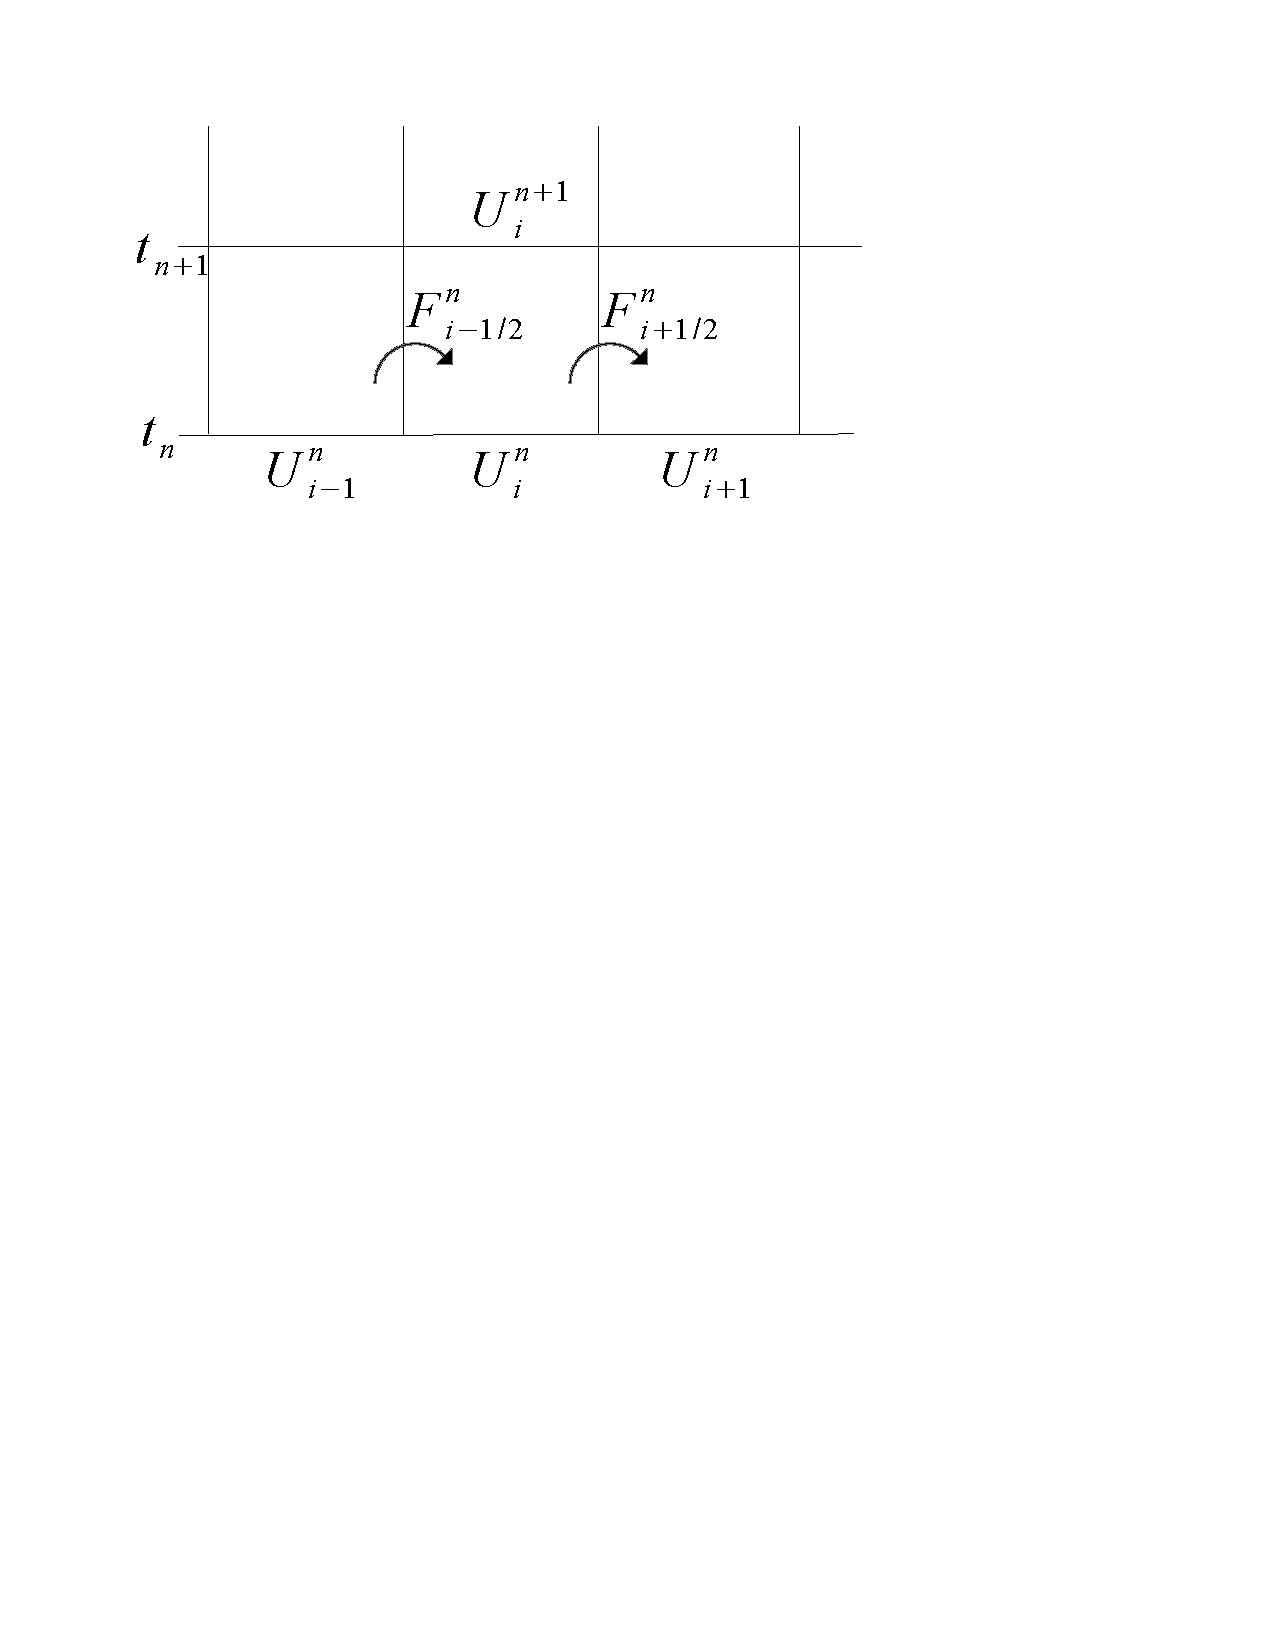
\includegraphics[trim= 20mm 195mm 0mm 30mm, clip]{flux_form.pdf}
\caption{A schematic of the fluxes for the finite volume method as indicated by \eqref{eqn:flux_form}.}
\end{figure}

The evolution of these volume-averaged quantities will depend only on the flux through the cell edges, so that
\begin{align}
\label{eqn:1D_semi_continuous}
\frac{d}{dt}\int_{C_i} u(x,t) dx = f(u(x_{i-1/2},t))-f(u(x_{i+1/2},t)).
\end{align}
We can then construct a time-stepping method where $\sum_i U_i^n\Delta x$ (the total `mass' of the system) is conserved from one time step $n$ to the next.

Let $F^n_{i-1/2} = \frac{1}{\triangle t}\int_{t^n}^{t^{n+1}} f(u(x_{i-1/2},t)) \, dt$.
Then
\begin{align*}
\int_{t^n}^{t^{n+1}} \left[ \frac{d}{dt}\int_{C_i} u(x,t)\, dx \right]
&{}= \int_{C_i} u(x,t^{n+1}) - u(x,t^{n})\, dx ,\\
&{ }= \triangle t \left(F^n_{i-1/2} - F^n_{i+1/2}\right).
\end{align*}

Thus, by integrating \eqref{eqn:1D_semi_continuous} in time, we may approximate the evolution of the cell (`volume') averages with the method
\begin{align}
\label{eqn:flux_form}
U_i^{n+1} = U_i^n - \frac{\Delta t}{\Delta x} \left(F^n_{i+1/2}-F^n_{i-1/2}\right).
\end{align}
where $U_i^n = \frac{1}{\triangle x} \int_{C_i} u(x,t^n) \, dt$.
% where
% \begin{gather}
% F_{i-1/2}^n = \frac{1}{\Delta t} \int_{t_n}^{t_{n+1}}f(u(x_{i-1/2},t))dt.
% \end{gather}
This formulation guarantees the conservation properties that are so desirable for conservation laws, if the time-averaged fluxes $F_{i-1/2}^n$ can be discretized in a natural way.

The key contribution of finite volume methods is the computation of $F_{i-1/2}^n$.
For a truly nonlinear $f(u)$ this can be rather complicated and messy, and typically will involve solving what is usually referred to as the Riemann problem for the conservation law.
The interested student can look at \cite{Le2002} for a very thorough introduction and discussion on the subject.
We will consider the linear problem in one dimension.
The analog to higher dimensions is obtained by considering the eigenvector decomposition of any linear system.
Nonlinear equations complicate things further.

\section*{The linear advection equation and upwinding}
The simplest conservation law describes the advection or transport of a quantity.
The PDE is given by
\begin{align}
u_t + au_x = 0, \label{eqn:fv_advection}
\end{align}
and describes the motion of a concentration of some constituent $u$ by a constant velocity one-dimensional `wind' $a>0$.
%(a slight generalization of this would be to consider $a=a(x)$, but the general concepts are exactly the same as those viewed here, just a more local consideration is necessary).
In higher dimensions this is an important problem in many fields, for example the transport of chemicals in the atmosphere and oceans, proper mixing of various properties in metallurgy, and the passing of information along a network.

Note that whenever $u(x,t)$ is a solution of the advection equation, then $u(x-at,t_0)$ (for any fixed $t_0$) is also a solution.
Thus, if $u(x,0) = u_0(x)$ then the solution for all time can be represented by $u(x,t) = u_0(x-at)$.
This is an important property of \eqref{eqn:fv_advection}, and gives a new meaning to the term advection: this equation merely takes the initial conditions and passively transports them with velocity $a$.

For this equation the computation of the flux appears straightforward: $F_{i-1/2}^n = a\overline{U}^n_{i-1/2}$ where the $\overline{U}^n_{i-1/2}$ refers to the time average of $U_{i-1/2}$ over the interval $t_n$ to $t_{n+1}$.
Let us determine how to approximate this time average.
% To understand how this might be done, note from Figure \ref{something} that for the advection equation with $a>0$ the flux that determines $U_i^{n+1}$ will be dependent on the value of $U_{i-1}^n$ so that it makes sense that we approximate the flux here as $F_{i-1/2}^n = aU_{i-1}^n$ (recall that the $U_i^n$ are cell averages of the continuous quantity $u(x)$).
Note from Figure \ref{fig:fv_LW_reconstruction} that when $a>0$ the flux that determines $U_i^{n+1}$ will be dependent on the value of $U_{i-1}^n$. Thus, one possibility is to approximate the flux by $F_{i-1/2}^n = aU_{i-1}^n$.
Using this approximation of the flux together with the flux differencing formula \eqref{eqn:flux_form} yields the first order upwind method, given by
\begin{align*}
U_i^{n+1} = U_i^n - \frac{a\Delta t}{\Delta x}\left(U_i^n-U_{i-1}^n\right).
\end{align*}
% (recall that the $U_i^n$ are cell averages of the continuous quantity $u(x)$).
% Similarly, if $a<0$ then $F_{i-1/2}^n = aU_{i}^n$.
% This is called the first order upwind method
% and gives a completely discretized version of the problem as \eqref{eq:flux_form} with
% \begin{align*}
% F_{i-1/2}^n = a^- U_i^n + a^+U_{i-1}^n,
% \end{align*}
% where $a^- = \min (a,0)$ and $a^+ = \max (a,0)$.
% Note that this formulation allows for an easy extension to the case where $a=a(x)$ is a more general function of $x$.
% From now on we will consider the simpler case where $a>0$ is constant.
% From now on we will consider $a>0$ only, the generalization to other cases is relatively straightforward.
% In either case, the flux differencing formula \eqref{eq:flux_form} yields
% \begin{align*}
% U_i^{n+1} = U_i^n - \frac{a\Delta t}{\Delta x}\left(U_i^n-U_{i-1}^n\right)
% \end{align*}
% for the upwind method.
Another way to derive the upwind method is to instead suppose that what we want to do is reconstruct $u(x)$ at each time step $n$ inside each cell $(x_{i-1/2},x_{i+1/2})$from the mean values in that cell and its surrounding neighbors. This reconstructed $\tilde{u}(x)^n$ is then defined piecewise for each cell $i$.
The solution at the next time step can be found as $\tilde{u}^{n+1}(x) = \tilde{u}^n(x-a\triangle t)$ which allows us to determine the fluxes $F^n_{i-1/2}$ once we have settled on a method for determining $\tilde{u}^n(x)$ in each cell.
The simplest approach is
\[\tilde{u}^n(x) = U_i^n \text{ for }x \in (x_{i-1/2},x_{i+1/2})\]
This leads to fluxes given by
\begin{align}
F_{i-1/2}^n &= \frac{a}{\triangle t}\int_{0}^{t_{n+1}-t_n} \tilde{u}^n(x_{i-1/2},t)\, dt , \\
&= \frac{a}{\triangle t}\int_{0}^{\triangle t} \tilde{u}^n(x_{i-1/2}-at)\, dt  ,\\
&= aU_{i-1}^n.\nonumber
\end{align}

\begin{figure}
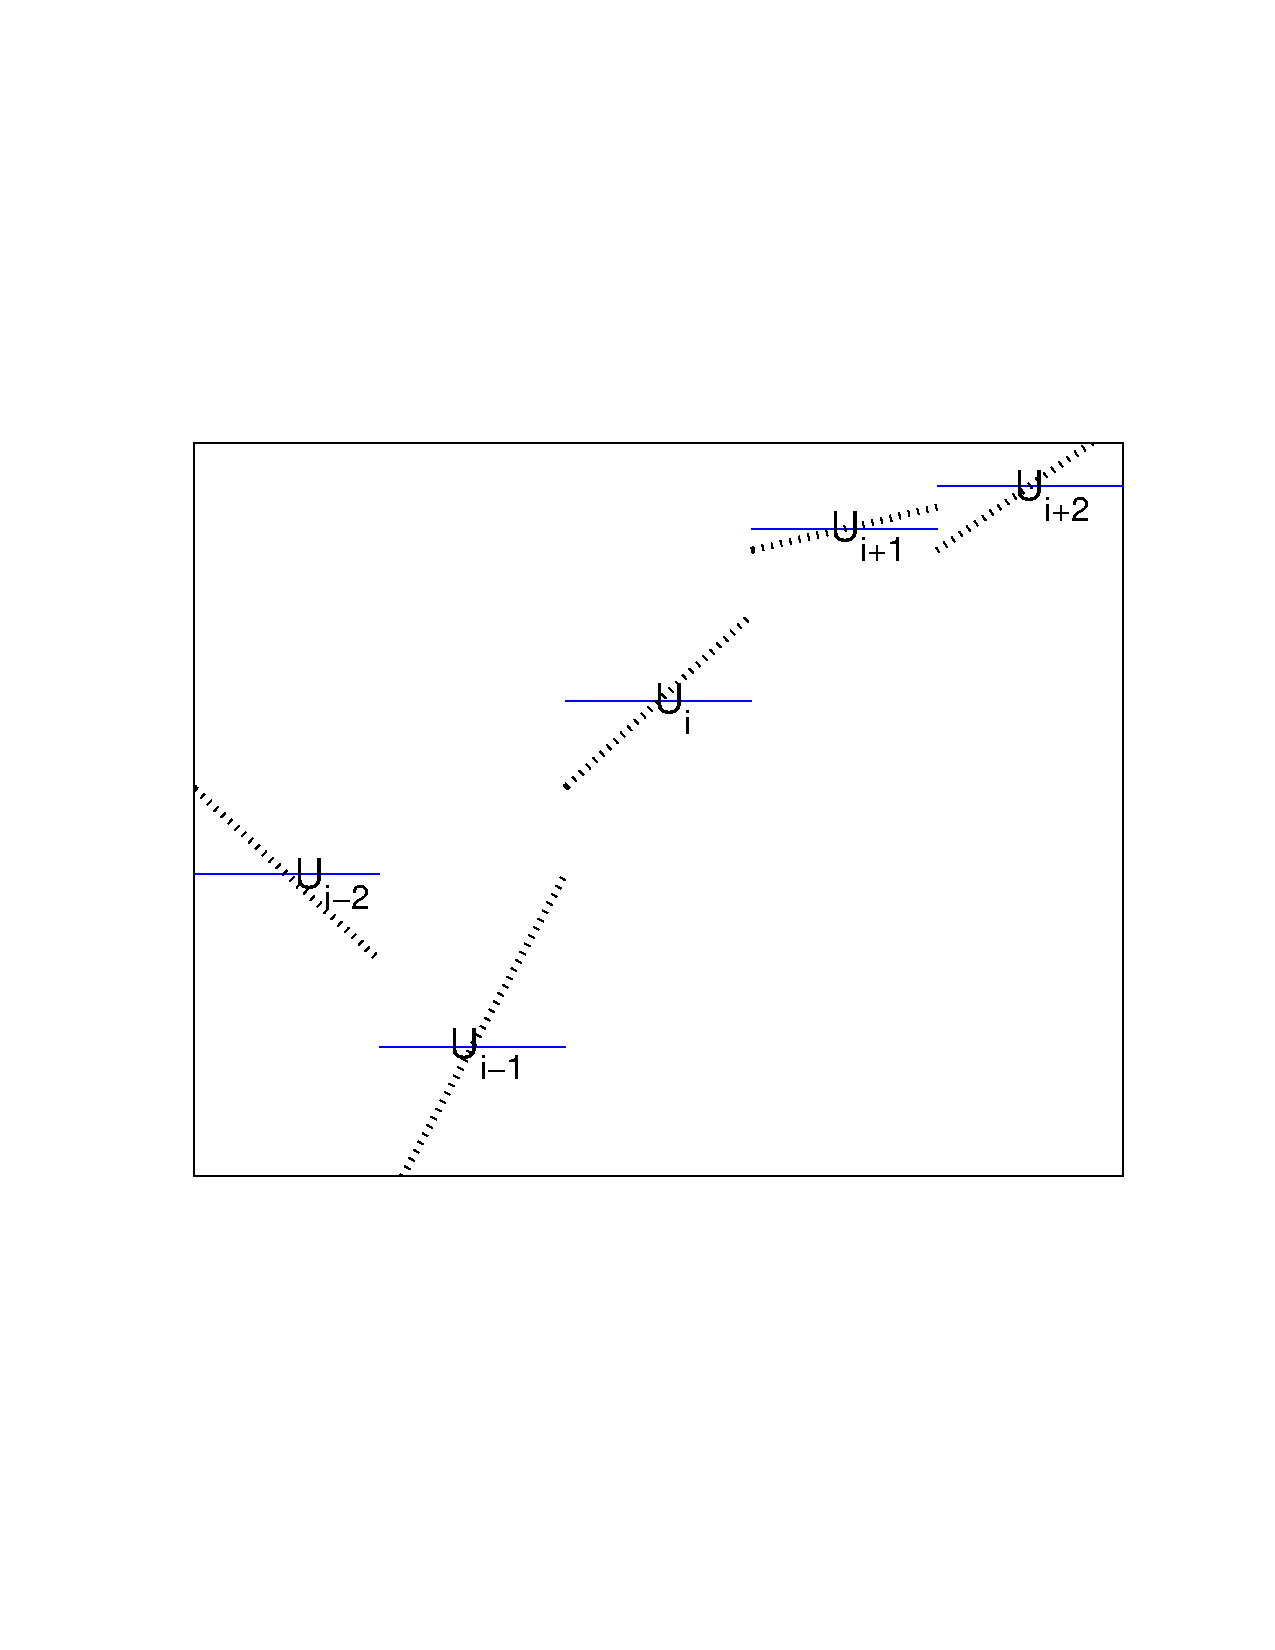
\includegraphics[width=\textwidth, trim = 20mm 65mm 20mm 65mm, clip]
{LW_reconstruction.pdf}
\caption{The piecewise linear reconstruction for the upwind and Lax-Wendroff methods.
The solid lines represent the simplest reconstruction of the cell averages leading to the upwind method, and the dashed lines are those whose slope is obtained via the Lax-Wendroff method.
Note that the LW method introduces a spurious maximum at $i+3/2$ (the cell edge between $U_{i+1}$ and $U_{i+2}$) and the minimum at $i-3/2$ will be unphysical exaggerated.
The upwind method avoids this difficulties, but clearly loses a significant amount of the available information.
This provides the motivation for the slope limiters.}
\label{fig:fv_LW_reconstruction}
\end{figure}

The following code solves the problem
\begin{align}
\begin{split}
	u_t +a u_x &= 0, \quad 0 < x < 1, \\
	u(x,t) &= f(x),\\
	u(0,t) &= u(1,t),
\end{split}\label{eqn:fv_exercise}
\end{align}
where $f$ represents a signal with two parts: one is smooth and the other is discontinuous.
Notice that this PDE has periodic boundary conditions.
Essentially we are evolving the signal around the unit circle.
This allows us to evolve the signal much further to test our numerical methods, since we only have to discretize the interval $[0,1]$ instead of a much larger domain.
To see how to implement the bounday conditions, consider a grid $0 = x_0< x_1< \ldots< x_{N-1}< x_N = 1$ of evenly spaced points.
Since $x_N = x_0$, it is sufficient to track $x_0, \ldots , x_{N-1}$.

\begin{lstlisting}
import numpy as np
from matplotlib import pyplot as plt
from math import floor

def upwind(u0, a, xmin, xmax, t_final, nt):
    """ Solve the advection equation with periodic
    boundary conditions on the interval [xmin, xmax]
    using the upwind finite volume scheme.
    Use u0 as the initial conditions.
    a is the constant from the PDE.
    Use the size of u0 as the number of nodes in
    the spatial dimension.
    Let nt be the number of spaces in the time dimension
    (this is the same as the number of steps if you do
    not include the initial state).
    Plot and show the computed solution along
    with the exact solution. """
    dt = float(t_final) / nt
    # Since we are doing periodic boundary conditions,
    # we need to divide by u0.size instead of (u0.size - 1).
    dx = float(xmax - xmin) / u0.size
    lambda_ = a * dt / dx
    u = u0.copy()
    for j in xrange(nt):
        # The Upwind method. The np.roll function helps us 
        # account for the periodic boundary conditions.
        u -= lambda_ * (u - np.roll(u, 1))
    # Get the x values for the plots.
    x = np.linspace(xmin, xmax, u0.size+1)[:-1]
    # Plot the computed solution.
    plt.plot(x, u, label='Upwind Method')
    # Find the exact solution and plot it.
    distance = a * t_final
    roll = int((distance - floor(distance)) * u0.size)
    plt.plot(x, np.roll(u0, roll), label='Exact solution')
    # Show the plot with the legend.
    plt.legend(loc='best')
    plt.show()

# Define the initial conditions.
# Leave off the last point since we're using periodic
# boundary conditions.
nx = 30
nt = nx * 3 // 2
x = np.linspace(0., 1., nx+1)[:-1]
u0 = np.exp(-(x - .3)**2 / .005)
arr = (.6 < x)  &  (x < .7 )
u0[arr] += 1.

# Run the simulation.
upwind(u0, 1.2, 0, 1, 1.2, nt)
\end{lstlisting}

Try running the previous code block with \li{nx} set to $30$, $60$, $120$, and $240$.
You will notice that the numerical solution diffuses with time.
It diffuses especially fast at the points of discontinuity.

\begin{comment}
Another way to derive the upwind method is to instead suppose that what we want to do is reconstruct $u(x)$ at each time step $n$ inside each cell $(x_{i-1/2},x_{i+1/2})$ from the mean values in that cell and its surrounding neighbors.
This reconstructed $\tilde{u}(x)^n$ is then defined piecewise for each cell $i$.
The solution at the next time step can be found as $\tilde{u}^{n+1}(x) = \tilde{u}^n(x-a\Delta t)$ which allows us to determine the fluxes $F_{i-1/2}^n$ once we have settled on a method for determining $\tilde{u}^n(x)$ in each cell.
The simplest approach is
\begin{gather*}
\tilde{u}^n(x) = U^n_i \mbox{ for } x \in (x_{i-1/2},x_{i+1/2}).
\end{gather*}
% This leads to fluxes given by
% \begin{gather}
% F_{i-1/2}^n = \frac{a}{\Delta t} \int_{t_n}^{t_{n+1}}\tilde{u}(x_{i-1/2}-a(t-t_n),t)dt = \frac{a}{\Delta t} \int_{t_n}^{t_{n+1}}U_i^n dt = aU_i^n.
% \end{gather}
In either case, we can see that using the flux differencing formula \eqref{eq:flux_form} that
\begin{gather}
U_i^{n+1} = U_i^n - \frac{a\Delta t}{\Delta x}\left(U_i^n-U_{i-1}^n\right)
\end{gather}
for the upwind method.
\end{comment}

\section*{Piecewise linear reconstruction and slope limiters}
The upwind method is formally only first order, and actually does relatively poorly in terms of actually transporting the initial data with velocity $a$.
You can notice from the example code that the upwind method has errors that are `diffusive' meaning that the initial data is diffused as time evolves, losing the peaks and fine details.
This is because the error for the upwind method is on the order of the second derivative of $u$ which is of a diffusive nature.
To get an improved method, consider a better reconstruction inside each cell, i.e.
\begin{gather}
\tilde{u}^n(x) = U_i^n + m_i^n(x-x_i) \mbox{ for } x \in (x_{i-1/2},x_{i+1/2})
\end{gather}
where the slope of this linear reconstruction $m_i^n$ is determined as a function of the neighboring cell averages at time $n$ and $U_i^n$ itself.
Then the flux is given by
\begin{align}
\begin{split}
F_{i-1/2}^n
&= \frac{a}{\triangle t}\int_{0}^{t_{n+1}-t_n} \tilde{u}^n(x_{i-1/2}-at)\, dt  ,\\
&= \frac{a}{\triangle t}\int_{0}^{\triangle t} U_{i-1}^n + m_i^n(x_{i-1/2} - at - x_i), \\
&= a \left( U_{i-1}^n + \frac{m_{i-1}^n}{2} (\triangle x - a \triangle t)\right).
\end{split}
\label{eqn:finite_volume_improved_flux}
\end{align}
One of the most natural approaches is to just estimate the slope depending on the cell $i$ and a neighboring cell $i+1$ or $i-1$.
This leads to two popular methods, the Lax-Wendroff method and the Beam-Warming method (that really is the name).
The Lax-Wendroff method has a slope chosen as
\begin{gather}
m_i^n = \frac{U^n_{i+1}-U_{i}^n}{\Delta x}.
\end{gather}
% This leads to
% \begin{gather}
% U_i^{n+1} = U_i^n - \frac{\Delta t}{2\Delta x} a \left(U_{i+1}^n-U_{i-1}^n\right) + \frac{1}{2}\left(\frac{\Delta t}{\Delta x}\right)^2 a^2 \left(U_{i-1}^n - 2U_i^n+U_{i+1}^n\right)
% \end{gather}
which it turns out is formally second-order accurate.
It turns out though that the errors for this method are dispersive, meaning that near very steep gradients, the method will generate very rapid oscillations (due to the third derivative of $u$ not being approximated accurately).
Another way to consider how these errors arise is to notice from Figure \ref{fig:fv_LW_reconstruction} that if the piecewise linear reconstruction is advocated by some positive wind $a$ then there will be places where the discontinuous nature of the reconstruction will introduce spurious maxima or minima into the solution.
These become the spurious waves seen in simulations using the Lax-Wendroff method.

A solution to this dilemma between balancing the diffusive and dispersive errors comes from constructing slopes $m_i^n$ that ensure no such non-monotonic transport takes place.
The basic idea is to constrain the slope so that the reconstructed piecewise linear function $\tilde{u}^n(x)$ will not generate unphysical extremal values when it is advocated by some finite wind $a$.
The Minmod limiter chooses the slope as 
\begin{gather}
m_i^n = minmod\left(\frac{U_i^n-U_{i-1}^n}{\Delta x},\frac{U_{i+1}^n-U_{i}^n}{\Delta x}\right)
\end{gather}
where
\begin{gather}
minmod(a,b) = \left\{\begin{array}{ccc}a  \mbox{ if } |a| < |b|  \mbox{ and } ab>0\\
b  \mbox{ if } |b|<|a|  \mbox{ and } ab>0\\ 0  \mbox{ if } ab < 0 .\end{array}\right.
\end{gather}

% \begin{itemize}
% \item Minmod limiter
% \begin{gather}
% m_i^n = minmod\left(\frac{U_i^n-U_{i-1}^n}{\Delta x},\frac{U_{i+1}^n-U_{i^n}}{\Delta x}\right)
% \end{gather}
% where
% \begin{gather}
% minmod(a,b) = \left\{\begin{array}{ccc}a  \mbox{ if } |a| < |b|  \mbox{ and } ab>0\\
% b  \mbox{ if } |b|<|a|  \mbox{ and } ab>0\\ 0  \mbox{ if } ab < 0 .\end{array}\right.
% \end{gather}
% \item Superbee limiter
% \begin{gather}
% m_i^n = maxmod(m^{(1)}_i,m^{(2)}_i)
% \end{gather}
% where the maxmod function selects $m^{(k)}_i$ with the larger modulus, and
% \begin{gather}
% m^{(1)}_i = minmod \left(\frac{U_{i+1}^n-U_i^n}{\Delta x},2\frac{U_i^n-U_{i-1}^n}{\Delta x}\right)\\
% m^{(2)}_i = minmod \left( 2\frac{U_{i+1}^n-U_i^n}{\Delta x},\frac{U_i^n-U_{i-1}^n}{\Delta x}\right).
% \end{gather}
% \item Monotonized central-difference limiter
% \begin{gather}
% m_i^n = minmod\left(\frac{U_{i+1}^n-U_{i-1}^n}{2\Delta x},2\frac{U_i^n-U_{i-1}^n}{\Delta x},2\frac{U_{i+1}^n-U_i^n}{\Delta x}\right)
% \end{gather}
% \end{itemize}

% \begin{problem}
% Code up the Superbee and Minmod %MC
% limiters for an advection problem with constant wind.
% Use different initial data that is smooth or has steep gradients (such as the square wave in the example code) to see which of the three limiters may be more optimal.
% \end{problem}

\begin{problem}
Implement the Lax Wendroff method and use it to solve \eqref{eqn:fv_exercise}.
Compare it to the upwind method for $N = 30, 60, 120$, and 240.
You should be able to tell that the Lax Wendroff method approximates the smooth portion of the signal much better, as it does not struggle with diffusion.
Unfortunately, it has some difficulty with the discontinuous portion, where unphysical oscillations are seen.
Recall that we saw something similar in the waves lab when there were discontinuous initial conditions.

Hint: Use equations \ref{eqn:finite_volume_improved_flux} and \ref{eqn:flux_form}.
\end{problem}

\begin{problem}
Implement the Minmod method and use it to solve \eqref{eqn:fv_exercise}.
Compare it to the upwind and Lax Wendroff methods for $N = 30, 60, 120$, and 240.
Be sure to vectorize the minmod operation.
\end{problem}

\begin{figure}
\centering
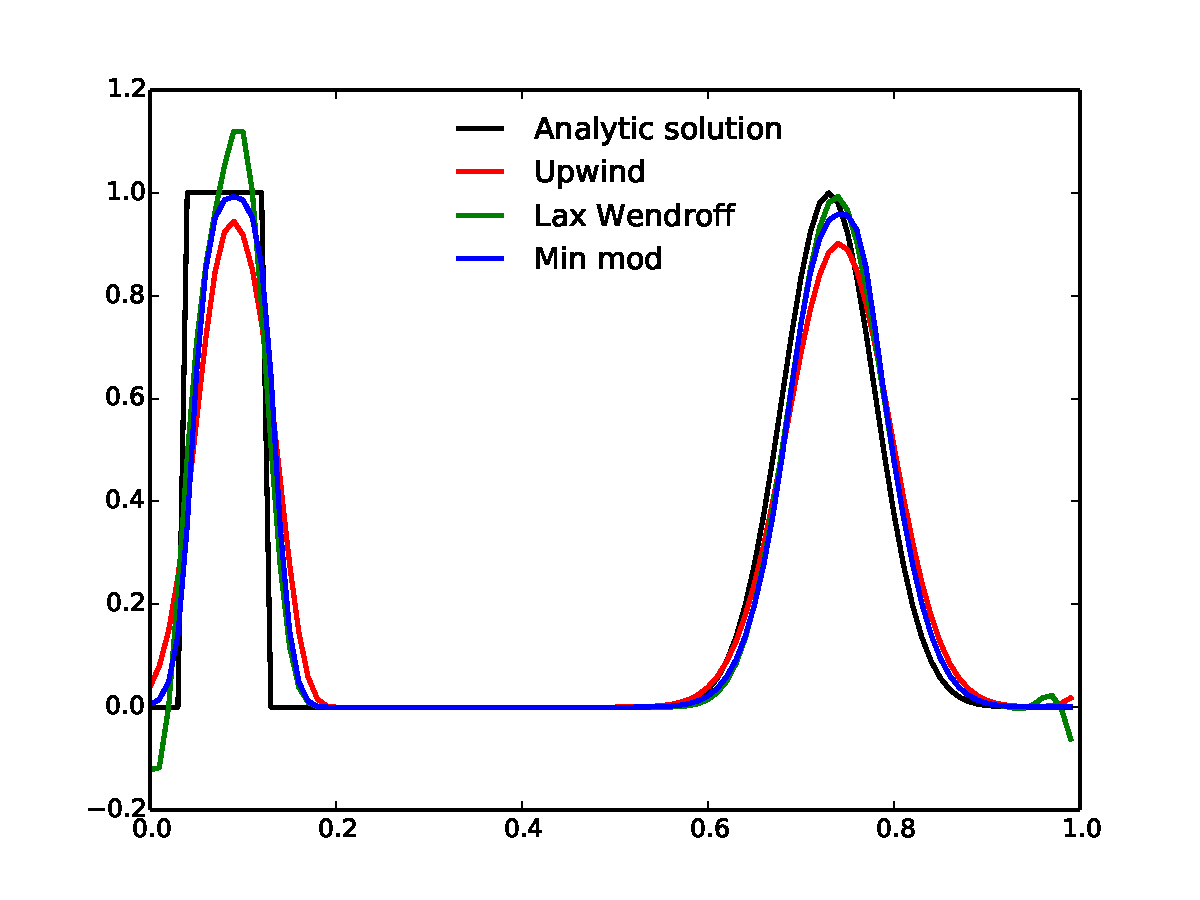
\includegraphics[width=\textwidth]{FiniteVolume_Comparisons.pdf}
\caption{Solutions of \eqref{eqn:fv_exercise} at time $t = 1.2$ using various methods.
Here the advection coefficient is $a = 1.2$, and there are  $N = 100$ subintervals in space, 150 subintervals in time.}
\label{fig:fv_Comparisons}
\end{figure}

\section*{Beyond piecewise linear reconstructions}
As you can imagine, using a linear approximation is not the only option.
There are a host of high order finite volume methods that consider polynomial reconstructions of $\tilde{u}^n$ inside each cell.
The key is then to use some nonlinear limiting technique that will ensure that when $\tilde{u}^n(x)$ is advocated that no new extrema are introduced.
Choosing the correct limiter for the given application then becomes an art unto itself.